%

\section{Logical Obstruction for Synchronous Message Passing Protocol}
\label{sec:obstructionSMP}

%
%


In this section, we argue the solvability of the consensus task by the
single-round synchronous message passing protocol, using partial product
update models.

In \cite{S1571:2001:HerlihyRajsbaumTuttle}, a precise topological analysis
has been given on the solvability of $k$-set agreement tasks by
synchronous message passing protocols of varying protocol rounds.
We demonstrate that the techniques developed in the previous sections can
be applied to reproduce a part of these results: The consensus task is
solvable by a single-round execution of the synchronous message passing
protocol if the number $n$ of agents in the system is $2$ or less;
otherwise, when $n>2$, it is unsolvable.

%
%
%

%
%
%
%
%
%
%
%
%
%

%
%
%
%
%

%
%
%
%
%


%
%

\subsection{Action model for the consensus task}
\label{subsec:consensustask}

%
%
%
%
%
%
%
%
%
%

%
%
%
%
%
%
%
%

%
%
%
%
%

%
%
%
%
%
%
%
%
%
%

The consensus task is specified by the following 
constraints on the input and output values of the agents.
\begin{itemize}
    \item \textbf{Agreement}:
          Every non-faulty agent must decide on the same output value;
    \item \textbf{Validity}:
          The agreed output value must be an input value to some of the agents in the system.
\end{itemize}


%
%
%
%

%

%
%

%
%
%
%
%
%
%
%
%
%
%
%

%
%

%
%

%

%
%
%
%

%

%
%

%

%
%

%
%
%
%

%
%
%
%
%
%
%
%
%
%
%
%

%
%
%
%
%
%
%
%
%
%
%
%




%
%
%
%
%
%
%
%
%
%
%

%
%
%

%
%
%
%
%
%
%
%
%
%


%
Without loss of generality, we may assume the set of possible inputs 
for the consensus task is $\{0,\ldots, n-1\}$, the set of agent ids. 

\begin{definition}[Partial product update model of the consensus task]\label{def:consensus}
    The consensus task is defined by a partial product update model $\ImProd{\cplI}{\actMf{T}}$,
    where  $\cplI$ is the input simplicial model and  
    $\actMf{T}=\anglpair{T, \relK{T}{}, \precond^T}$ is the action model consisting of:
\begin{itemize}
    \item The set of actions $T= \Ag = \{0,\ldots, n-1\}$;
    \item The family of indistinguishability relations $\{ \relK{T}{a} \}_{a\in\Ag}$
          defined by  $v \relK{T}{a} v'$ iff $v=v'$;
    \item The precondition defined by 
          $\precond^T (v) =\bigvee_{a\in \Ag} \Pinput{a}{v}$
          for each action $v\in T$.
\end{itemize}
\end{definition}

An action in $v\in T$ stands for a single output value unanimously decided by all live agents.
Each agent can distinguish any pair of distinct actions in $T$, since all agents know 
the agreed value.   
The precondition $\precond^T(v)$ guarantees the validity condition
of the consensus task, that is, the agreed value~$v$ must be the input
to some agent~$a$. 



%
%

\subsection{Solvability of the consensus task with 2 agents}
\label{subsec:2consensus}

Let us show that the consensus task is solvable, when $n=2$. %
(The case $n=1$ is trivial.)
%
%
%
%
%

%

%
%
%
%
%
%
%
%
%

Remember that the input simplicial model $\cplI$ for $2$ agents consists 
of four facets $X_{00}, X_{01}, X_{10}, X_{11}$, 
where $X_{ij}= \{(0,i), (1,j)\}$ for each $i,j \in \{0,1\}$.  
The consensus task is then given by 
the partial product update model 
$\ImProd{\cplI}{\actMf{T}}=\anglpair{W, \sim,  L}$ consisting of:
\begin{itemize}
    \item $W= \{(\{X_{ij}\}, 0)\mid i\neq 1 \text{ or } j\neq 1\}\cup \{(\{X\}, 1)\mid i\neq 0 \text{ or } j\neq 0\}$;
    \item The indistinguishability relation defined by  
    $(\{X\}, v) \relK{}{a} (\{X'\}, v')$ iff           $X\relK{\cplI}{a} X'$ and $v=v'$, for each $a\in\Ag$;
    \item $L\bigl((\{X\}, v)\bigr)=\labSM^{\cplI} (X)$.
\end{itemize}
The underlying complex of $\ImProd{\cplI}{\actMf{T}}$ is illustrated 
in Figure~\ref{fig:consensusPPU_2}.
Note that the complex is pure, meaning that every agent $a\in\Ag$ is alive in every world of the model.
%
%

%

\begin{figure}[ht]
    \centering
    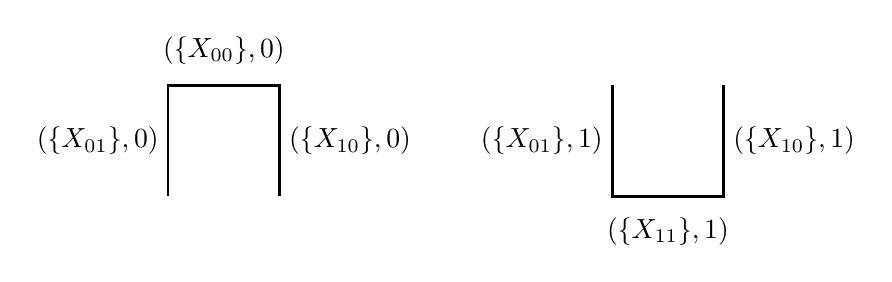
\begin{tikzpicture}[scale=1.41]
        \draw[thick](0, 0)--(0, 1)--(1, 1)--(1, 0);
        \draw[thick](4, 1)--(4, 0)--(5, 0)--(5, 1);

        \draw(0, 0)node{{\Large $\nodeR$}};
        \draw(0, 1)node{{\Large $\nodeW$}};
        \draw(1, 1)node{{\Large $\nodeR$}};
        \draw(1, 0)node{{\Large $\nodeW$}};

        \draw(0, 0.5)node [anchor=east]{$(\{X_{01}\}, 0)$};
        \draw(0.5, 1.1)node [anchor=south]{$(\{X_{00}\}, 0)$};
        \draw(1, 0.5)node[anchor=west]{$(\{X_{10}\}, 0)$};

        \draw(4, 1)node{{\Large $\nodeW$}};
        \draw(4, 0)node{{\Large $\nodeR$}};
        \draw(5, 0)node{{\Large $\nodeW$}};
        \draw(5, 1)node{{\Large $\nodeR$}};


        \draw(4.0, 0.5)node [anchor=east]{$(\{X_{01}\}, 1)$};
        \draw(4.5, -0. 1)node[anchor=north]{$(\{X_{11}\}, 1)$};
        \draw(5, 0.5)node[anchor=west]{$(\{X_{10}\},  1)$};
    \end{tikzpicture}
    \caption{The partial product update model $\ImProd{\cplI}{\actMf{T}}$ of the consensus task for $2$ agents}
    \label{fig:consensusPPU_2}
\end{figure}
%






%
%
%

%
    %
    %
    %
    %
    %
    %
    %
    %
    %
    %
    %
    %
    %
    %
    %
    %
    %
    %
    %
    %
    %
    %
    %
    %

    Next, let us consider the partial product update model 
    $\ImProd{\cplI}{\MP{\cplI}}$ for the synchronous message passing protocol, 
    where $\MP{\cplI}$ is the action model for $2$~agents. 
    Remember that the inputless action model for $2$~agents 
    is given by $\ActOneSMP=\anglpair{\MPpA{2},\MPprel{2}}$,
    where $\MPpA{2}=\{\clos{\emptyset},  \clos{\{0<1\}},$ $\clos{\{1<0\}}\}$. 
    For brevity, let us write $t_{\emptyset}$, $t_0$, and $t_1$ for the posets
    $\clos{\emptyset}$,  $\clos{\{0<1\}}$, and $\clos{\{1<0\}}$, respectively.
    Topologically, these posets correspond to the facets in the impure
    simplicial complex illustrated in Figure~\ref{fig:inputless_n2}.
        
        %
        %
        %
        %
        %
        %
        %
    

\begin{figure}[ht]
    \begin{minipage}[b]{.44\linewidth}
        \centering
        \begin{tikzpicture}
            \draw[thick](-0.5,0)--(0.5,0);

            \draw(-1.5,0)node{{\Large $\nodeR$}};
            \draw(-1.5,0.5)node{$t_0$};

            \draw(-0.5,0)node{{\Large $\nodeW$}};
            \draw(0.5,0)node{{\Large $\nodeR$}};

            \draw(1.5,0)node{{\Large $\nodeW$}};
            \draw(1.5,0.5)node{$t_1$};

            \draw(0,0.5)node{$t_{\emptyset}$};

        \end{tikzpicture}
        \vspace*{4em}
        \subcaption{Inputless action model $\ActOneSMP$}
        \label{fig:inputless_n2}
    \end{minipage}\hfil%
    \begin{minipage}[b]{.55\linewidth}
        \centering
        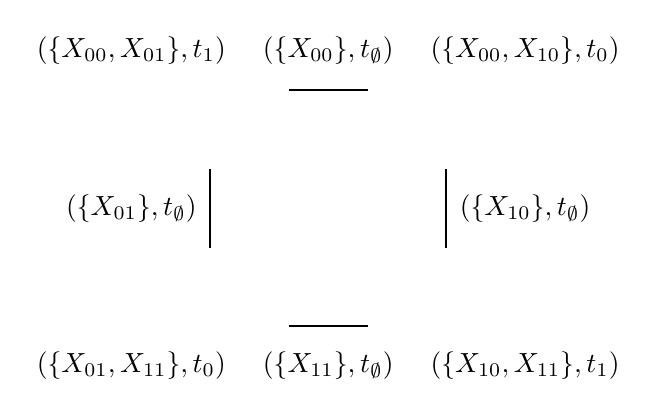
\begin{tikzpicture}
            \draw[thick](0, 1)--(0, 2);
            \draw[thick](1, 3)--(2, 3);
            \draw[thick](1, 0)--(2, 0);
            \draw[thick](3, 1)--(3, 2);

            \draw(0, 0)node{{\Large $\nodeR$}};
            \draw(0, 2)node{{\Large $\nodeR$}};
            \draw(1, 3)node{{\Large $\nodeR$}};
            \draw(2, 0)node{{\Large $\nodeR$}};
            \draw(3, 3)node{{\Large $\nodeR$}};
            \draw(3, 1)node{{\Large $\nodeR$}};

            \draw(0, 1)node{{\Large $\nodeW$}};
            \draw(0, 3)node{{\Large $\nodeW$}};
            \draw(1, 0)node{{\Large $\nodeW$}};
            \draw(3, 2)node{{\Large $\nodeW$}};
            \draw(3, 0)node{{\Large $\nodeW$}};
            \draw(2, 3)node{{\Large $\nodeW$}};

            \draw(1. 5, 3. 5)node{$(\{X_{00}\}, t_{\emptyset})$};
            \draw(1. 5, -0. 5)node{$(\{X_{11}\}, t_{\emptyset})$};
            \draw(-1, 3. 5)node{$(\{X_{00}, X_{01}\},  t_1)$};
            \draw(4, 3. 5)node{$(\{X_{00}, X_{10}\}, t_0)$};
            \draw(-1, 1. 5)node{$(\{X_{01}\}, t_{\emptyset})$};
            \draw(4, 1. 5)node{$(\{X_{10}\}, t_{\emptyset})$};
            \draw(-1, -0. 5)node{$(\{X_{01}, X_{11}\}, t_0)$};
            \draw(4,  -0. 5)node{$(\{X_{10}, X_{11}\},  t_1)$};
        \end{tikzpicture}
        \subcaption{Action model $\MP{\cplI}$}
        \label{fig:inputfull_n2}
    \end{minipage}
    \caption{Action model of the synchronous message passing protocol for $2$ agents}
    \label{fig:actModels_impure}
\end{figure}


%
%
%
%

Following Definition~\ref{def:SMP}, we obtain the action model 
$\MP{\cplI}=\anglpair{\MPA{\cplI}, \MPrel{\cplI}, \MPprecond{\cplI}}$ consisting of:
%
%
%
%
\begin{itemize}
    \item The set of actions 
    \[
        \MPA{\cplI}=
                \{(\{X_{ij}\}, t_{\emptyset})\mid i,j\in\{0,1\} \}
                \cup\{(\{X_{0j}, X_{1j}\},  t_0)\mid j\in \{0, 1\}\}\cup \{(\{X_{i0}, X_{i1}\},  t_1)\mid i\in \{0, 1\}\};\]
    \item The family of indistinguishability relations defined by  
    $(\ActEquiv{t}{X}, t)\MPrel{\cplI}_a (\ActEquiv{t'}{X'},t')$ iff 
    $(\ActEquiv{t}{X}, t) =(\ActEquiv{t'}{X'},t')$ and $t\sim^{\ActOneSMP}_a t'$;
    %
    %
            %
            %
    \item The labeling $\MPprecond{\cplI} \bigl((\ActEquiv{t}{X} , t)\bigr)=\bigvee \{\bigwedge \labSM^{\cplI}(X')\mid X' \in \ActEquiv{t}{X}\}$.
\end{itemize}
%
%
The corresponding topological structure of this action model is illustrated by the simplicial complex
in Figure~\ref{fig:inputfull_n2}.


    %
    %
    %
    %

    %
    %
    %


    Combining $\cplI$ and $\MP{\cplI}$, we obtain a partial product update model of
    the synchronous message passing protocol $\ImProd{\cplI}{\MP{\cplI}}$ for $2$ agents,
    where its Kripke frame has a topological structure isomorphic to that of the action model $\MP{\cplI}$
    and the labeling  $L^{\ImProd{\cplI}{\MP{\cplI}}}$
    on the worlds of the Kripke frame is given by:
    \[
        L^{\ImProd{\cplI}{\MP{\cplI}}}\bigl((\ActEquiv{t}{X},  t)\bigr)= \bigcap \{\labSM^{\cplI}(X')\mid X' \in \ActEquiv{t}{X}\}.
    \]

    %
    %
    %
    %
    %
    %
    %
    %
    %
    %
    %
    %

    Observe that $\ImProd{\cplI}{\actMf{T}}$ corresponds to a complex comprising of
    two disconnected subcomponents, one for the output $0$ and the other for $1$
    and that $\ImProd{\cplI}{\MP{\cplI}}$ corresponds to
    a collection of discrete facets, none of which are connected.
    It is easy to devise a morphism $\delta:
    \ImProd{\cplI}{\MP{\cplI}}\to\cplI\{\actMf{T}\}$   that satisfies the
    condition~\eqref{eq:kripsolve} in Section~\ref{subsec:tasksolv} for
    task solvability.
    For instance, such a morphism~$\delta$ is given by:
    \begin{align*}
        \delta\bigl((\{X_{11}\},  t_{\emptyset})\bigr)  & {} = \bigsat{\{0,1\}}{(\{X_{11}\}, 1)},                           \\
        \delta\bigl((\{X_{ij}\}, t_{\emptyset})\bigr)   & {} =\bigsat{\{0,1\}}{(\{X_{ij}\}, 0)} \quad  (i\neq 1 \text{ or } j \neq 1), \\
        \delta\bigl((\ActEquiv{t_0}{X_{ij}},  t_0)\bigr) & {} =\bigsat{\{1\}}{(\{X_{ij}\},j)},                               \\
        \delta\bigl((\ActEquiv{t_1}{X_{ij}},  t_1)\bigr) & {} =\bigsat{\{0\}}{(\{X_{ij}\},  i)}.
    \end{align*}
    %
    %
    %
%

\begin{theorem} \label{th:consSolvable2Ags}
    Suppose we have a system of $2$ agents with $\Ag=\{0,1\}$. Then
    the consensus task is solvable by
    the single-round synchronous message passing protocol.
\end{theorem}



%
%

\subsection{Unsolvability of the consensus task with 3 agents}
\label{subsec:unsolvecons3}

%
%
%

The consensus task is not solvable by the synchronous message passing protocol,
when the number $n$ of agents is $3$ or greater.
This is because, in contrast to the case where $n$ is $2$ or less, the
resulting partial product update model of the protocol is more tightly
connected in a topological sense.

To demonstrate this topological intuition in partial epistemic models,
we first examine the case $n=3$, where the 
partial product update model $\ImProd{\cplI}{\MP{\cplI}}$ of the 
synchronous message passing protocol is an 
impure $2$-dimensional complex. 
%

    %
    %
    %
    Let us define a guarded positive formula $\Phi_3\in \ModLang_{\Modalfont{K}, \Palive}^+$ by
    \[
        \Phi_3 \equiv \ModK{2} \ModK{1}\ModK{2}\varphi_0 \vee \ModK{0}\ModK{2}\ModK{0} \varphi_1 \vee \ModK{1}\ModK{0}\ModK{1} \varphi_2,
    \]
    where 
    $\varphi_i \equiv \bigvee_{a\in\Ag} \Palive(a)\Rightarrow \Pinput{a}{i}$ for $i=0,1,2$.

    %


    We claim that $\Phi_3$ is a logical obstruction.
    That is, $\Phi_3$ is valid in $\cplI\{\actMf{T}\}$ but not valid in $\ImProd{\cplI}{\ActSMP}$,
    where $\actMf{T}$ is the action model for the consensus task
    and $\ActSMP$ is the action model for the synchronous message passing protocol, for $3$~agents.

    The input simplicial complex $\cplI$ for $3$ agents has 
    an underlying pure $2$-dimensional complex and we write
    $X_{ijk}$ to denote a facet $\{(0,i), (1,j), (2,k)\}$ of the complex, where $i,j,k \in \{0, 1, 2\}$.
    The labeling on a facet is defined by $\labSM^{\cplI}(X_{ijk})=\{\Pinput{0}{i}, \Pinput{1}{j}, \Pinput{2}{k}\}$.
    %
    %
    %
    The action model of the consensus task $\actMf{T}=\anglpair{T, \sim^T, \precond^T}$
    is defined similarly  as in Section~\ref{subsec:2consensus}, except that
    the set of actions $T= \{0, 1, 2\}$ consists of the three possible outputs $0$, $1$, and $2$.


    %
    %
    %
    %
    %
    %

    %
    %
    %
    %
    %
    %
    %
    %
    %

    The partial product update model $\ImProd{\cplI}{\actMf{T}}$ of the consensus task
    has an underlying complex, pure of dimension~$2$.
    This means that 
    $\Palive(a)$ is true for every agent $a\in\Ag$ in every world of $\ImProd{\cplI}{\actMf{T}}$
    and therefore $\varphi_i$ 
    is equivalent to $\precond^T (i)=\bigvee_{a\in\Ag}\Pinput{a}{i}$ 
    for each action $i\in \{0,1,2\}$. 
    (Remember that $T=\Ag= \{0,\ldots, n-1\}$.)
    %
    %
    %
    %
    %
    %
        %
    %
    %
        By the definition, $\ImProd{\cplI}{\actMf{T}}, (\preEqClass{v}{X}, v)\models \varphi_v$ holds.
    %
    Since $(\preEqClass{v}{X}, v) \relK{T}{a} (\preEqClass{v'}{X'}, v')$ 
    implies $v=v'$ for every $a\in\Ag$,  either of the disjuncts 
    $\ModK{2} \ModK{1}\ModK{2}\varphi_0$, $\ModK{0}\ModK{2}\ModK{0} \varphi_1$, or  
    $\ModK{1}\ModK{0}\ModK{1} \varphi_2$ holds. 
    Therefore $\Phi_3$ is
    a valid formula in $\ImProd{\cplI}{\actMf{T}}$. 

    %
    %
    %

    %
    %
    %
    %
    %
    %
    %
    %
    %

    We then discuss the remaining half, i.e., $\Phi_3$ is invalid in
    the partial product update model of the synchronous message passing protocol.
    Remember that the inputless action model $\ActOneSMP$ for $3$ agents 
    has an impure $2$-dimensional complex given in Figure~\ref{fig:3_protKripSmpOne}
    as the underlying complex, and that each facet in $\ActOneSMP$ is represented
    by a poset. 
    %
    %
    %
    %
    %
    %
    %
    %
    %
    %
    %

    %
    %

    %
    %
    %

    %
    %

    %
    %

    %
    %

    %
    %
    %

    %

    %
    %

    %
    %
    %
    %
    %
    %
    %


    %
    %
    %
    %
    %
    %
    %
    %
    %
    %
    %

    As we have seen in Section~\ref{subsec:constActModel}, 
    we can derive the action model $\MP{\cplI}$ by making 
    copies of the inputless model $\ActOneSMP$ for each input facet of the input model
    and then pasting them appropriately.
    To show the unsolvability of the consensus task, it suffices to
    consider pasting the copies for two facets $X_{012}$ and $X_{112}$.
    This  results in a subcomplex of $\MP{\cplI}$ given in
    Figure~\ref{fig:actionmodelMPI},   which merges the result of actions
    on the input   facet $X_{012}$ (the left half of the picture) and that
    on $X_{112}$     (i.e., the right half).
    %
    %
    %
    %
    %
    %
    In the figure, some facets are designated by the corresponding actions:
    $t_0= (\ActEquiv{\clos{\emptyset}}{X_{012}}, \clos{\emptyset})$,
    $t_1= (\ActEquiv{u_1}{X_{012}}, u_1)$, %
    $t_2= (\ActEquiv{u_1}{X_{112}}, u_1)$, %
    $t_3= (\ActEquiv{\clos{\emptyset}}{X_{112}},  \clos{\emptyset})$, and
    $t_4 = (\ActEquiv{u_2}{X_{012}}, u_2)$,
    where 
    $u_1=\clos{\{ 0< 1 \}}=\clos{\{ \nodeW < \nodeR \}}$ and
    $u_2=\clos{\{ 0<1, 0<2 \}}=\clos{\{ \nodeW< \nodeR, \nodeW < \nodeB \}}$.
    As already discussed in Section~\ref{subsec:constActModel}, 
    the two copies of the complex of $\ActOneSMP$ are merged via 
    the facet designated by $t_4$, since
    $\ActEquiv{u_2}{X_{012}}=\ActEquiv{u_2}{X_{112}}$.

    %
    %
    %
    %
    %
    %
    %
    %
    %

    %
    %
    %
    %
    %


    \begin{figure}[ht]
        %
        \centering
        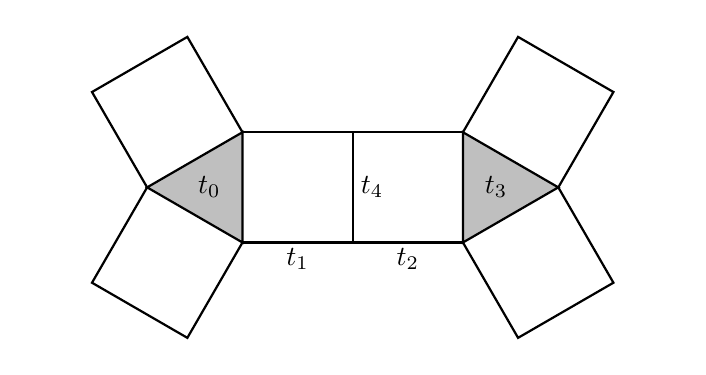
\begin{tikzpicture}[scale=0.7]
            \draw[fill=lightgray,  thick](2, 1)--(2, -1)--(3. 73, 0)--cycle;
            \draw(2. 6, 0)node{$t_3$};

            \draw[fill=lightgray,  thick](-2, 1)--(-2, -1)--(-3. 73, 0)--cycle;
            \draw(-2. 6, 0)node{$t_0$};

            \draw[thick](2, 1)--(-2, 1);
            \draw(-1, -1. 3)node{$t_1$};
            \draw(1, -1.3)node{$t_2$};

            \draw[thick](2, -1)--(-2, -1);
            \draw[thick](0, 1)--(0, -1);
            \draw(0.35, 0)node{$t_4$};

            \draw[thick](2, 1)--(3, 2. 73)--(4. 73, 1. 73)--(3. 73, 0);
            \draw[thick](2, -1)--(3, -2. 73)--(4. 73, -1. 73)--(3. 73, 0);

            \draw[thick](-2, 1)--(-3, 2. 73)--(-4. 73, 1. 73)--(-3. 73, 0);
            \draw[thick](-2, -1)--(-3, -2. 73)--(-4. 73, -1. 73)--(-3. 73, 0);

            \draw(0, 1)node{{\Large $\nodeB$}};
            \draw(0, -1)node{{\Large $\nodeR$}};

            \draw(0, 2.73)node{{\Large $\nodeR$}};
            \draw(0, -2.73)node{{\Large $\nodeB$}};
            \draw(-5.73, 0)node{{\Large $\nodeW$}};
            \draw(5.73, 0)node{{\Large $\nodeW$}};



            \draw(2, 1)node{{\Large $\nodeR$}};
            \draw(2, -1)node{{\Large $\nodeB$}};
            \draw(3. 73, 0)node{{\Large $\nodeW$}};
            \draw(3, 2. 73)node{{\Large $\nodeW$}};
            \draw(4. 73, 1. 73)node{{\Large $\nodeR$}};
            \draw(3, -2. 73)node{{\Large $\nodeW$}};
            \draw(4. 73, -1. 73)node{{\Large $\nodeB$}};


            \draw(-2, 1)node{{\Large $\nodeR$}};
            \draw(-2, -1)node{{\Large $\nodeB$}};
            \draw(-3. 73, 0)node{{\Large $\nodeW$}};
            \draw(-3, 2. 73)node{{\Large $\nodeW$}};
            \draw(-4. 73, 1. 73)node{{\Large $\nodeR$}};
            \draw(-3, -2. 73)node{{\Large $\nodeW$}};
            \draw(-4. 73, -1. 73)node{{\Large $\nodeB$}};
        \end{tikzpicture}
        \caption{A subcomplex of the action model $\MP{\cplI}$ that merges the actions on $X_{012}$ and $X_{112}$}
        \label{fig:actionmodelMPI}
    \end{figure}


    We obtain the partial product update model $\ImProd{\cplI}{\MP{\cplI}}$ 
    for the synchronous message passing protocol by combining $\cplI$ with $\MP{\cplI}$.
    %
    We note that $\ImProd{\cplI}{\MP{\cplI}}$
    has an isomorphic partial epistemic frame with that of the action model $\MP{\cplI}$.
    (See Appendix~\ref{prop:protocolEq} for the formal discussion of this fact.)
    Therefore, without loss of generality,
    we may regard $\ImProd{\cplI}{\MP{\cplI}}$
    as a partial epistemic model $\anglpair{\MPA{\cplI}, \MPrel{\cplI},L^{\MP{\cplI}}}$,
    where $\anglpair{\MPA{\cplI}, \MPrel{\cplI}}$ is the Kripke frame of $\MP{\cplI}$
    and $L^{\MP{\cplI}}$ is a labeling on the worlds of $\MPA{\cplI}$:
    \[
        L^{\MP{\cplI}}\bigl((\ActEquiv{t}{X},  t)\bigr)= \bigcap \{\labSM^{\cplI}(X')\mid X' \in \ActEquiv{t}{X}\}.
    \]

%
%
%
%


    %
    %
    %
    %
    %
    %


    %
    %
    %

    %
    %
    %
    %
    %

    Now we show that $\Phi_3$ is invalid in 
    the partial product update model $\ImProd{\cplI}{\MP{\cplI}}$.
    We claim that $\Phi_3$ is false in the world $t_0$ in Figure~\ref{fig:actionmodelMPI}.
    %
    %

    %

    %
    %
    %
    %
    %
    %
    %
    %
    %
    %
    %
    %
    %
    %

    %
    %

    %
    %
    %
    %
    %
    %

    %
    %
    %
    %
    %
    %
    %
    %
    %
    %


    %
    %
    %
    %
    %
    %


    From Figure~\ref{fig:actionmodelMPI}, it is easy to see that
    the facet $t_0$ is connected with $t_3$ via
    $t_0 \MPrel{\cplI}_2 t_1 \MPrel{\cplI}_1 t_2 \MPrel{\cplI}_2 t_3$.
    We show $\ImProd{\cplI}{\MP{\cplI}}, t_0 \not\models \ModK{2}\ModK{1}\ModK{2} \varphi_0$, 
    by traversing the above path in reverse order.
    %
    In $t_3$, all agents are alive, that is,
    $\ImProd{\cplI}{\MP{\cplI}},  t_3 \models \Palive(a) $
    for every $a\in \Ag$.
    Since $L^{\ActSMP}(t_3)=  \{\Pinput{0}{1}, \Pinput{1}{1}, \Pinput{2}{2}\}$,
    $\varphi_0 \equiv \bigvee_{a\in\Ag} \Palive(a)\Rightarrow \Pinput{a}{0}$ is false,
    i.e., $\ImProd{\cplI}{\MP{\cplI}},  t_3 \not\models \varphi_0$.
    %
    Since $t_3 \MPrel{\cplI}_2 t_2$,
    this implies that $\ImProd{\cplI}{\MP{\cplI}},  t_2 \not\models \ModK{2}\varphi_0$.
    Repeating this by traversing $t_2 \MPrel{\cplI}_1 t_1$ and then
    $t_1 \MPrel{\cplI}_2 t_2$,
    we obtain
    $\ImProd{\cplI}{\MP{\cplI}},  t_2 \not\models \ModK{2}\ModK{1}\ModK{2}\varphi_0$.
    This shows that $\ModK{2}\ModK{1}\ModK{2}\varphi_0$ is an invalid formula in
    $\ImProd{\cplI}{\MP{\cplI}}$.

    Due to the symmetry of the partial product update model $\ImProd{\cplI}{\MP{\cplI}}$,
    we can similarly show the invalidity of the remaining disjuncts in $\Phi_3$.
    Therefore $\Phi_3$ is invalid in $\ImProd{\cplI}{\MP{\cplI}}$.

%
%
%
%

\begin{theorem}\label{thm:unsolvecons3}
    For a system of $3$ agents with $\Ag=\{0,1,2\}$, the consensus task is not solvable by
    the single-round synchronous message passing protocol.
\end{theorem}



\subsection{Unsolvability of the consensus task, general case}
\label{subsec:unsolveconsgeneral}

%

We show the unsolvability for the general case, where the number of agents is $3$ or greater.
%
The proof is almost the same as that for $3$~agents, but we have to argue
the connectivity in a complex of higher dimension. 
Below we present a logical obstruction for the general case and
discuss the connectivity symbolically on the formal description of actions.


%
%
%

\begin{theorem}\label{thm:unsolveconsn}
    For a system with $\Ag=\{0,\cdots, n-1\}$ ($n\geq3$), 
    the consensus task is not solvable by the single-round synchronous message passing protocol.
\end{theorem}

\begin{proof}
    Let us define a guarded positive formula $\Phi_n$ ($n\geq 3$) by:
    \[
        \Phi_n \equiv \bigvee_{i\in \{0, \cdots,  n-1\}} \ModK{(i+2)\bmod n}\ModK{(i+1)\bmod n}\ModK{(i+2)\bmod n} \varphi_i,
    \]
    where $\varphi_i \equiv \bigvee_{a\in\Ag} \Palive(a)\Rightarrow \Pinput{a}{i}$
    for each $i$ ($0\leq i\leq n-1$).

    We claim that $\Phi_n$ is a logical obstruction.
    Let $\cplI$ be the input model, $\actMf{T}$ be the action model of the consensus task,
    $\MP{\cplI}$ be the action model of the synchronous message passing protocol, 
    each defined for $n$ agents.
    We also let $\ImProd{\cplI}{\actMf{T}}$
    and $\ImProd{\cplI}{\MP{\cplI}}$ be the partial product update models
    for the task and the protocol, respectively.

    %
    %
    %
    %
    %
    %


    %
    %
    %

    By Theorem~\ref{thm:LOTheorem}, it suffices to
    show that $\Phi_n$ is valid in $\ImProd{\cplI}{\actMf{T}}$
    but is invalid in $\ImProd{\cplI}{\MP{\cplI}}$.
    The validity of $\Phi_n$ is $\ImProd{\cplI}{\actMf{T}}$ is similarly shown
    as we have demonstrated in Section~\ref{subsec:unsolvecons3}.

    %
    %

    Let us show that $\Phi_n$ is invalid in 
    $\ImProd{\cplI}{\MP{\cplI}}=\anglpair{\MPA{\cplI}, \MPrel{\cplI},L^{\ActSMP}}$. 
    Similarly as in Section~\ref{subsec:unsolvecons3}, by symmetry,
    it suffices to show that $\ModK{2} \ModK{1} \ModK{2} \varphi_0$
    is false in some world of $\ImProd{\cplI}{\MP{\cplI}}$.
    We show that $\ImProd{\cplI}{\MP{\cplI}}, (\ActEquiv{\clos{\emptyset}}{X},  \clos{\emptyset})
        \not\models \ModK{2} \ModK{1} \ModK{2} \varphi_0$,
    where $X$ is a facet of $\cplI$ that is uniquely identified by the labeling
    $\labSM^{\cplI} (X)=\{\Pinput{i}{i}\mid 0\leq i \leq n-1\}$.


    %
    %
    %
    %
    %
    %
    %
    %
    %
    %
    %
    %

    Let us define $X'$ be the facet of $\cplI$ that is uniquely determined by
    the labeling $\labSM (X') =\{\Pinput{0}{1}\} \cup \{\Pinput{i}{i}\mid 1\leq i \leq n-1\}$.
    We show that
    $(\ActEquiv{\clos{\emptyset}}{X},  \clos{\emptyset})$
    and
    $(\ActEquiv{\clos{\emptyset}}{X'},  \clos{\emptyset})$
    are connected along the following path:
    \[
        (\ActEquiv{\clos{\emptyset}}{X}, \clos{\emptyset})\MPrel{\cplI}_2
        (\ActEquiv{\clos{\{0< 1\}}}{X},  \clos{\{0<1\}})\MPrel{\cplI}_1
        (\ActEquiv{\clos{\{0< 1\}}}{X'}, \clos{\{0<1\}}) \MPrel{\cplI}_2
        (\ActEquiv{\clos{\emptyset}}{X'},  \clos{\emptyset}).
    \]
    %
    %
    %
    %
    %
    %
    
    To show $(\ActEquiv{\clos{\emptyset}}{X}, \clos{\emptyset})\MPrel{\cplI}_2
        (\ActEquiv{\clos{\{0< 1\}}}{X},  \clos{\{0<1\}})$, 
    it suffices to show $\clos{\emptyset} \relK{\ActOneSMP}{2} \clos{\{0<1\}}$, 
    which immediately follows from $2\not\in \lo(\clos{\emptyset})\cup \lo(\clos{\{0<1\}})$.
    %
    %
    %
    The proof of 
    $(\ActEquiv{\clos{\{0< 1\}}}{X'}, \clos{\{0<1\}}) \MPrel{\cplI}_2
    (\ActEquiv{\clos{\emptyset}}{X'},  \clos{\emptyset})$ is similar.
    %
    For $(\ActEquiv{\clos{\{0< 1\}}}{X},  \clos{\{0<1\}})\MPrel{\cplI}_1 (\ActEquiv{\clos{\{0< 1\}}}{X'}, \clos{\{0<1\}})$, 
    since $X\not\sim^{\cplI}_a X'$ if and only if $a\neq 0$,  
    it suffices to show that $\clos{\{0<1\}}\relK{\ActOneSMP}{1} \clos{\{0<1\}}$, 
    which  follows from $1 \not\in \Lo(\clos{\{0<1\}})$.

    %
    %
    


    %
    %
    %
    %
    %
    %
    %
    %
    %
    %
    %
    %
    %
    %
    %
    %


    %

    %
    %
    %
    
    All agents are alive in $(\ActEquiv{\clos{\emptyset}}{X'},  \clos{\emptyset})$, that is,
    $\MP{\cplI},  (\ActEquiv{\clos{\emptyset}}{X'},  \clos{\emptyset}) \models \Palive(a)$ 
    holds   for every $a\in \Ag$.
    Furthermore, 
    $L^{\ImProd{\cplI}{\MP{\cplI}}} \bigl((\ActEquiv{\clos{\emptyset}}{X'},  \clos{\emptyset})\bigr)
    = \{ \Pinput{0}{1} \} \cup \{ \Pinput{i}{i} \mid 1\leq i \leq n-1  \}$.
    These imply $\ImProd{\cplI}{\MP{\cplI}}, (\ActEquiv{\clos{\emptyset}}{X'},  \clos{\emptyset}) \not\models
    \varphi_0$. %
    Traversing the above path in reverse order, we sequentially obtain 
    $\ImProd{\cplI}{\MP{\cplI}},(\ActEquiv{\clos{\{0< 1\}}}{X'}, \clos{\{0<1\}})$ $\not\models \ModK{2}\varphi_0$, then
    $\ImProd{\cplI}{\MP{\cplI}}, (\ActEquiv{\clos{\{0< 1\}}}{X}, \clos{\{0<1\}}) \not\models \ModK{1}\ModK{2}\varphi_0$, 
    and finally
    $\ImProd{\cplI}{\MP{\cplI}}, (\ActEquiv{\clos{\emptyset}}{X},  \clos{\emptyset}) \not\models \ModK{2}\ModK{1}\ModK{2}\varphi_0$. 
    This proves that $\ModK{2}\ModK{1}\ModK{2}\varphi_0$ is invalid in  $\ImProd{\cplI}{\MP{\cplI}}$.

    %
    %
    %
    %
    %
    %
    %

    %
    %


    %
    %
    %
    %
    %
    %
    %
    %
    %
    %
    %
    %
    %
    %
    %
    %
    %
    %
    %

    %
    %
    %
    %
    %
    %
    %
    %
    %

    Consequently, by Theorem~\ref{thm:LOTheorem},
    we conclude that the consensus task is not solvable by the synchronous message passing protocol,
    if the number of agents is $3$ or greater.
\end{proof}
